\section{TCP and Wireless}

Wireless is less reliable than cable, and losses are common. In TCP though,
every loss is treated as a congestion. This causes:
\begin{itemize}
\item Multiple cwnd\footnote{Congestion window} reductions
\item Disconnections due to timeouts
\item Bandwidth waste
\end{itemize}

This has also an impact on multi-hop paths: it takes twice the time to
transmit data with two hops, because is not possible to forward the message at
the same time, but you have to wait, otherwise you'll end up with a collision.
Increasing number of hops beyond three allows simultaneous transmission on more
than one link, however, degradation continues due to contentions between TCP
data and ACKs traveling in opposite directions.

With movement, throughput degrades, because there is a possibility of link
breakage and route failure.

To solve these issues, we could adopt a different way of seeing the network:
\textit{traditional TCP}, \textit{connection split} and
\textit{pure end-to-end} connection.

\subsection{Traditional TCP} The protocol is not aware of wireless link, and
possible timeouts are treated like congestions. Implementations:
\begin{itemize}
\item TCP Reno
\item TCP New Reno
\item TCP Vegas
\item TCP SACK
\end{itemize}

\subsection{Connection split} The network is split, having local
retransmission and quick actions on the wireless link.
Examples:
\begin{itemize}
\item I-TCP
\item M-TCP
\item Proxy
\item Snoop Protocol
\end{itemize}

\subsubsection{Snoop Protocol} In this protocol, there is a tower with a big
buffer keeping a list of ACKs: it handles dupAcks/lost packages, without
stopping the sender from sending new data to the tower.
Considerations:
\begin{itemize}
\item Pro:
  \begin{itemize}
  \item Local (and timely) loss recovery
  \item End-to-end semantics preservation (almost)
  \end{itemize}
\item Cons:
  \begin{itemize}
  \item Requires a little RTTs on the wireless link
  \item No guarantee against long disconnections
  \end{itemize}
\end{itemize}

\subsection{Pure end-to-end} In this protocol, the sender is aware of the wireless
link. There are endless number of implementations of end-to-end protocols:
\begin{itemize}
\item TCP WestWood/WestWood+
\item TCP Cubic
\item TCP Hybla
\item TCP High speed
\item \dots
\end{itemize}

\subsubsection{TCP WestWood} This TCP version involves changes only to the
sender side of the connection, and not to everyone. It's useful for satellite
communications.
 
Flow control is based on an estimation of the eligible bandwidth (BWE). TCP
WestWood can perform an estimation determined from ACK internal-arrival times
and info in ACKs regarding amounts of bytes delivered.
The \mKeyword{rate estimation} enhance congestion control, and is used by the
sender to properly set $cwnd$ and $SSTHRESH$ after a packet loss (either a
three dupAcks or a timeout). Rate estimation is based on three formulas.
\begin{equation}
  RE_k = a_k \cdot RE_{k-1} + (1 - a_k) \cdot \left( \frac{b_k + b_{k-1}}{2}
  \right)
  \label{eq:tcpw:ef}
\end{equation}

This formula calculate the filter. In particular, this formula is quick to
compute, and allows to set proportions like: 75\% $RE_{k-1}$ (the portion of the
previous volume) and 25\% of samples. Obviously, it takes some time to have a
good estimation of the bandwidth.
To calculate the samples, the formula is:
\begin{equation}
b_k = \frac{\sum_{t_j > t_k-T} d_j }{T} = \frac{ACK\ seen}{Time\ Passed}
\end{equation}

\begin{figure}[t]
  \centering
  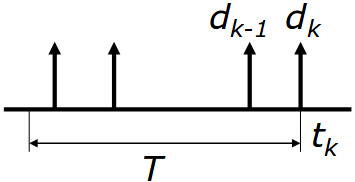
\includegraphics[scale=0.3]{TCPWRE}
  \caption[Graphical $b_k$ representation]{Representative schema of how $b_k$ is
    calculated}
  \label{fig:tcpw:TCPWRE}
\end{figure}

Note that this formula is based on $T$ (indicating typically the RTT): on one
hand having a small $T$ it means being more aggressive at the rate estimation,
on the other hand having a big $T$ it means being more conservative.


At the end, the filter is calculated another time:
\begin{equation}
a_k = \frac{2t - \Delta t_k}{2t + \Delta t_k}
\end{equation}
it's important to consider that his formula is difficult to compute and slows
down the whole formula,~\ref{eq:tcpw:ef}.

With the way~\ref{eq:tcpw:ef} is calculated, the value is fine-tuned over time.

\paragraph*{Handling losses in TCP WestWood} When three dupAcks occurs
we have that $SSTHRESH = BWE \cdot RTT_{min}$ and if the cwnd is greater than
the SSTHRESH we set $cwnd=SSTHRESH$.
Otherwise if a timeout occurs we have $SSTHRESH = BWE \cdot RTT_{min}$ but the
cwnd becomes equals to 1.

\paragraph*{Final considerations}
\begin{itemize}
\item Pro:
  \begin{itemize}
    \item bandwidth estimation done at the sender side
    \item code modifications only at the sender side
  \end{itemize}
\item Cons:
  \begin{itemize}
  \item wrong bandwidth estimation over asymmetric links
  \item no specific mechanism to handle disconnections
  \item problems with fairness \& friendliness\footnote{\textbf{Fairness}:
    One flow with the \textbf{same} protocol $\rightarrow$ same
    bandwidth usage.
    
    \textbf{Friendliness}: One flow with \textbf{different} protocols
    $\rightarrow$ same bandwidth usage.}
  \end{itemize}
\end{itemize}

\begin{figure}[t]
\centering
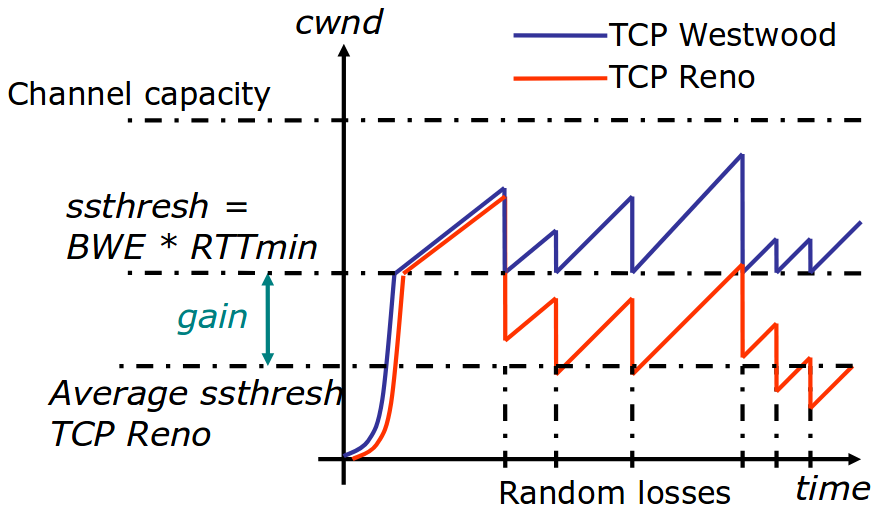
\includegraphics[scale=0.30]{TCPWestWood}
\caption[TCP WestWood vs TCP Reno]{A comparison between TCP WestWood and TCP Reno}
\label{fig:tcpw:tcpwwvstcpr}
\end{figure}
